\documentclass[12pt,twoside,space]{ctexart}
\usepackage{NEMT}
\begin{document}\zihao{5}
\juemi
\biaoti{高考数学}
\fubiaoti{一卷}
{\heiti 注意事项}
\begin{enumerate}[itemsep=-0.3em,topsep=0pt]
\item 答卷前,考生务必将自己的姓名和准考证号填写在答题卡上。
\item 回答选择题时,选出每小题答案后,用铅笔把答题卡对应题目的答案标号涂黑。如需改动,用橡皮擦干净后,再选涂其它答案标号。回答非选择题时,将答案写在答题卡上。写在本试卷上无效。
\item 考试结束后,将本试卷和答题卡一并交回。
	请认真核对监考员在答题卡上所粘贴的条形码上的姓名、准考证号与您本人是否相符。
\end{enumerate}
\section{选择题:本题共1个小题,共6分}
\begin{enumerate}[itemsep=0.2em,topsep=0pt]
\item
一道考题有4个答案,要求学生将其中的一个正确答案选择出来。某考生知道正确答案的概率为$\frac{1}{3}$,若不知正确答案,学生会乱猜。在乱猜时,4个答案被选择的概率均为$\frac{1}{4}$,如果他答对了,则他确实知道正确答案的概率是
\begin{tasks}(4)\task $\frac{1}{3}$ \task $\frac{2}{3}$ \task $\frac{3}{4}$ \task $\frac{1}{4}$ 
\end{tasks}
\end{enumerate}
\section{解答题:本题共4个小题,共38分}
\begin{enumerate}[itemsep=0.2em,topsep=0pt]
\item
1.已知抛物线$ \Gamma $:$ y^2=2px(p>0) $的焦点为$ F $、$ P $是抛物线$ \Gamma $上一点,且在第一象限,满足$ (2,2) $  (1)求抛物线$ \Gamma $的方程;    (2)已知经过点$ A $$ (3,2) $的直线交抛物线$ \Gamma $于$ M、N $两点,经过定点$ B $$ (3,-6) $和$ M $的直线与抛物线$ \Gamma $交于另一点$ L $  , 问直线$ NL $是否恒过定点,如果过定点,求出该定点,否则说明理由.
\item
如图,抛物线$ y=\frac{1}{5}x^2-\frac{16}{5} $与x轴交与A,B两点,顶点为C,点P在抛物线上,且位于x轴下方。已知P(1,-3),B(4,0),若点D是抛物线上的一点,满足$ \angle DPO=\angle POB $,求点D的坐标。
\begin{figure}[htbp]
                      \centering
                      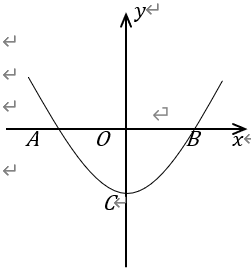
\includegraphics[width=10em]{288793-1630484678-2.jpg}
\end{figure}\\[-1.5em]
\item
在$\triangle ABC$中,角$A,B,C$对应的边分别为$a,b,c$且$b=1,c=\sqrt{3},\angle C=\frac{2}{3}\pi.$(1)求$cosB$的值.(2)求$a$的值
\item
在$\triangle ABC$中,角$A,B,C$对应的边分别为$a,b,c$且$b=1,c=\sqrt{3},\angle C=\frac{2}{3}\pi.$(1)求$cosB$的值.(2)求$a$的值
\end{enumerate}

\clearpage
\end{document}
\documentclass{article}
\usepackage{pdfpages}
\usepackage[paperwidth=39.5cm,paperheight=27.2cm]{geometry}
\begin{document}
\includepdf[pages=1-6,nup=2x1]{dibajiefeishujuesaijuanzi.pdf}
\end{document}
doublepages